\documentclass[varwidth=\maxdimen]{standalone}

\usepackage[dvipdfmx]{graphicx}
\usepackage{multirow}
\usepackage{array}
\usepackage{booktabs}
\usepackage{makecell}

\begin{document}
\begin{table}
  \centering
  \begin{tabular}{ccccc}
    \multicolumn{4}{c}{\textbf{3elt}}                                   \\
    \raisebox{-.5\height}{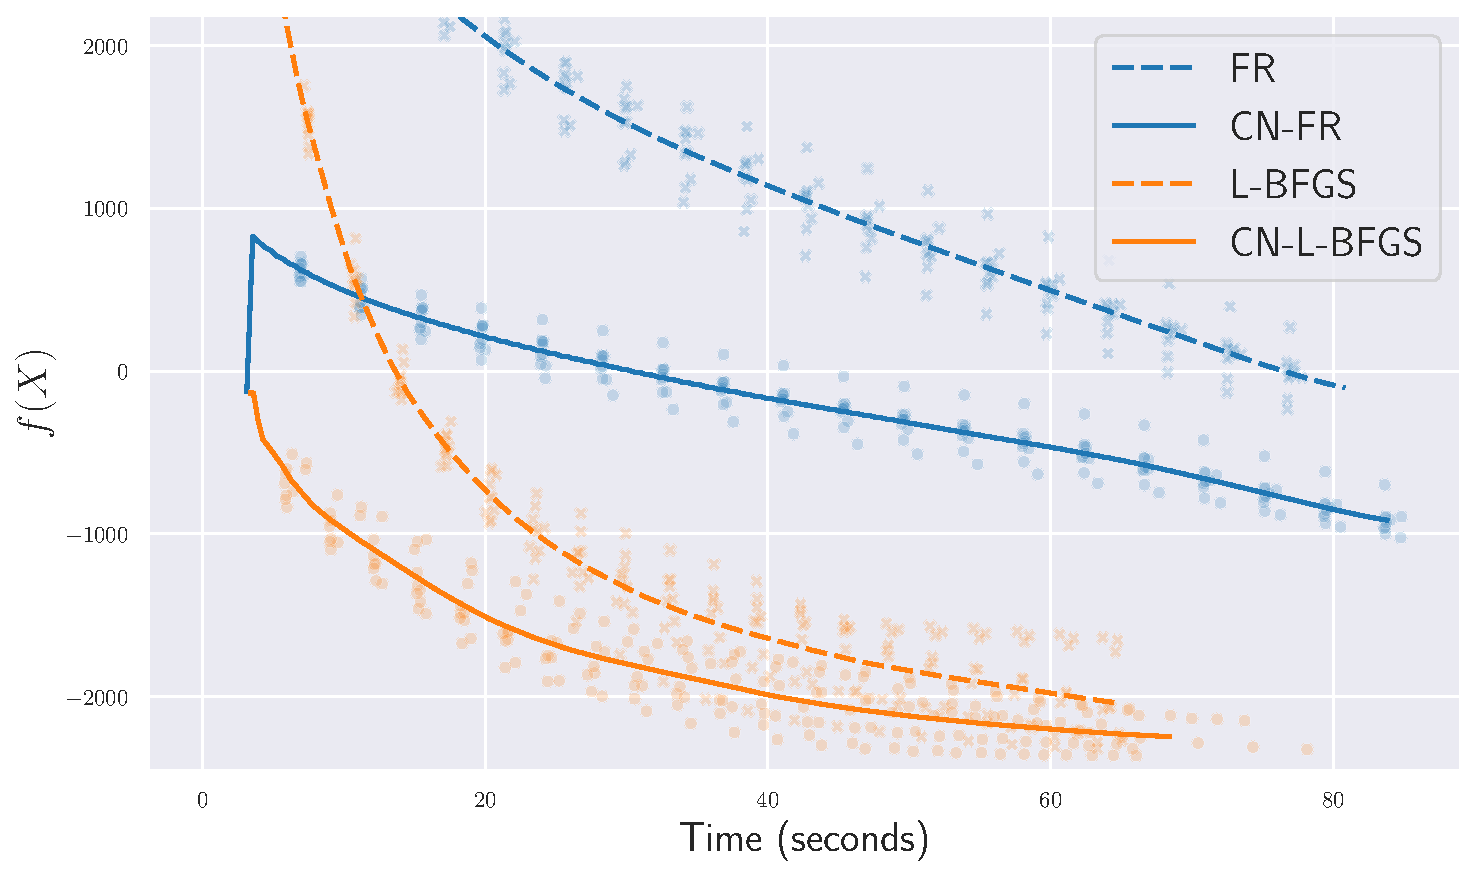
\includegraphics[width=6cm]{plot/3elt.pdf}} &
    \makecell{\scriptsize{FR}                                           \\[-0.2em]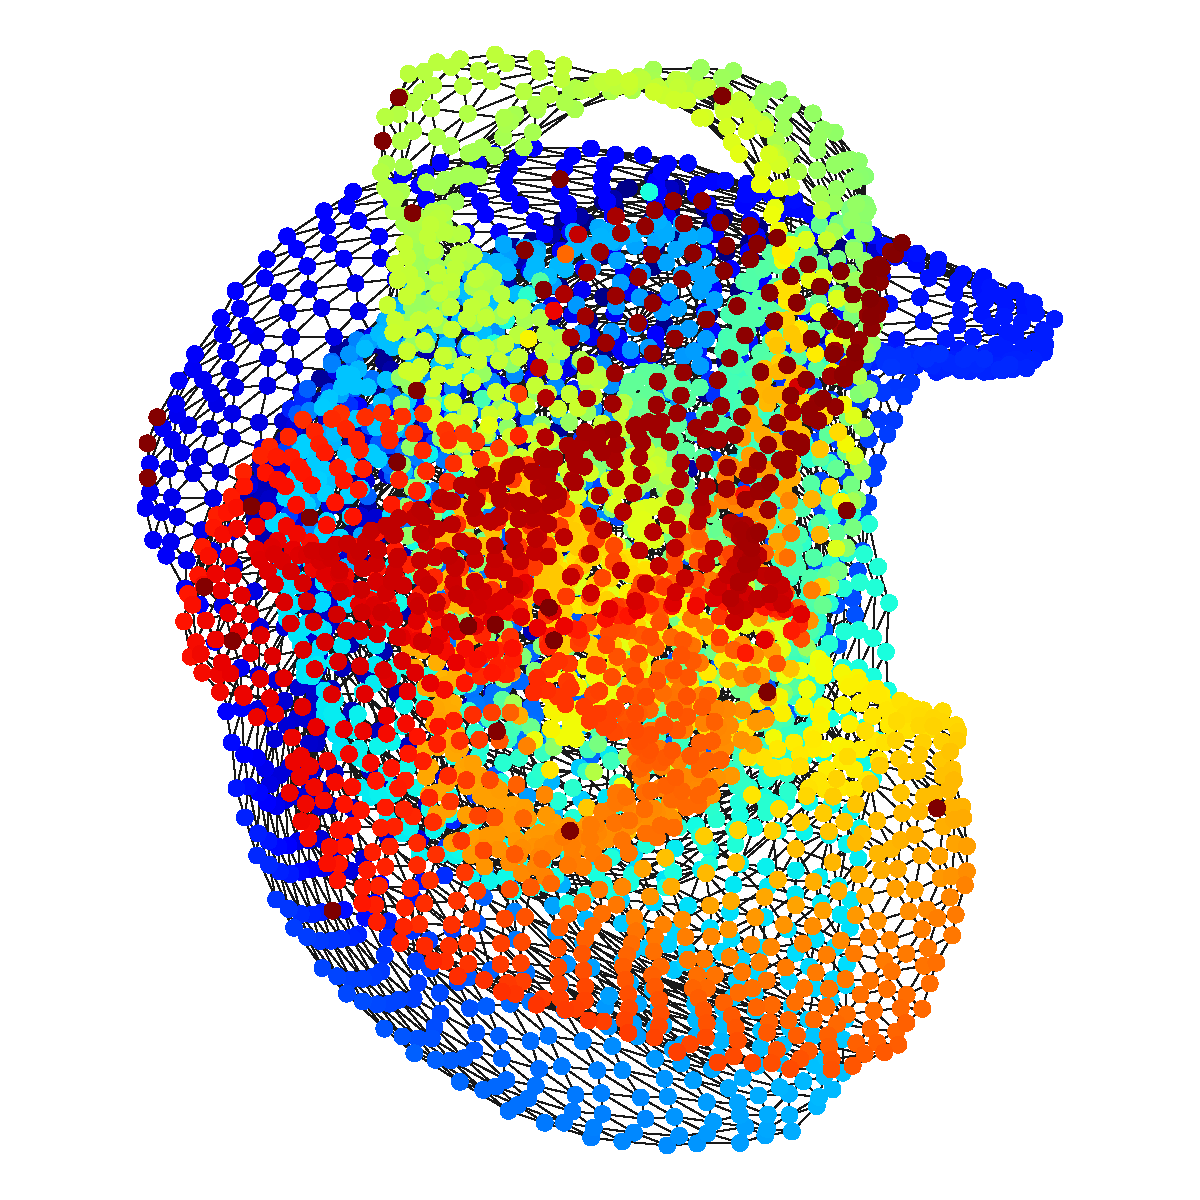
\includegraphics[width=2.5cm]{viz/3elt_FR.pdf}} &
    \makecell{\scriptsize{L\_BFGS}                                      \\[-0.2em]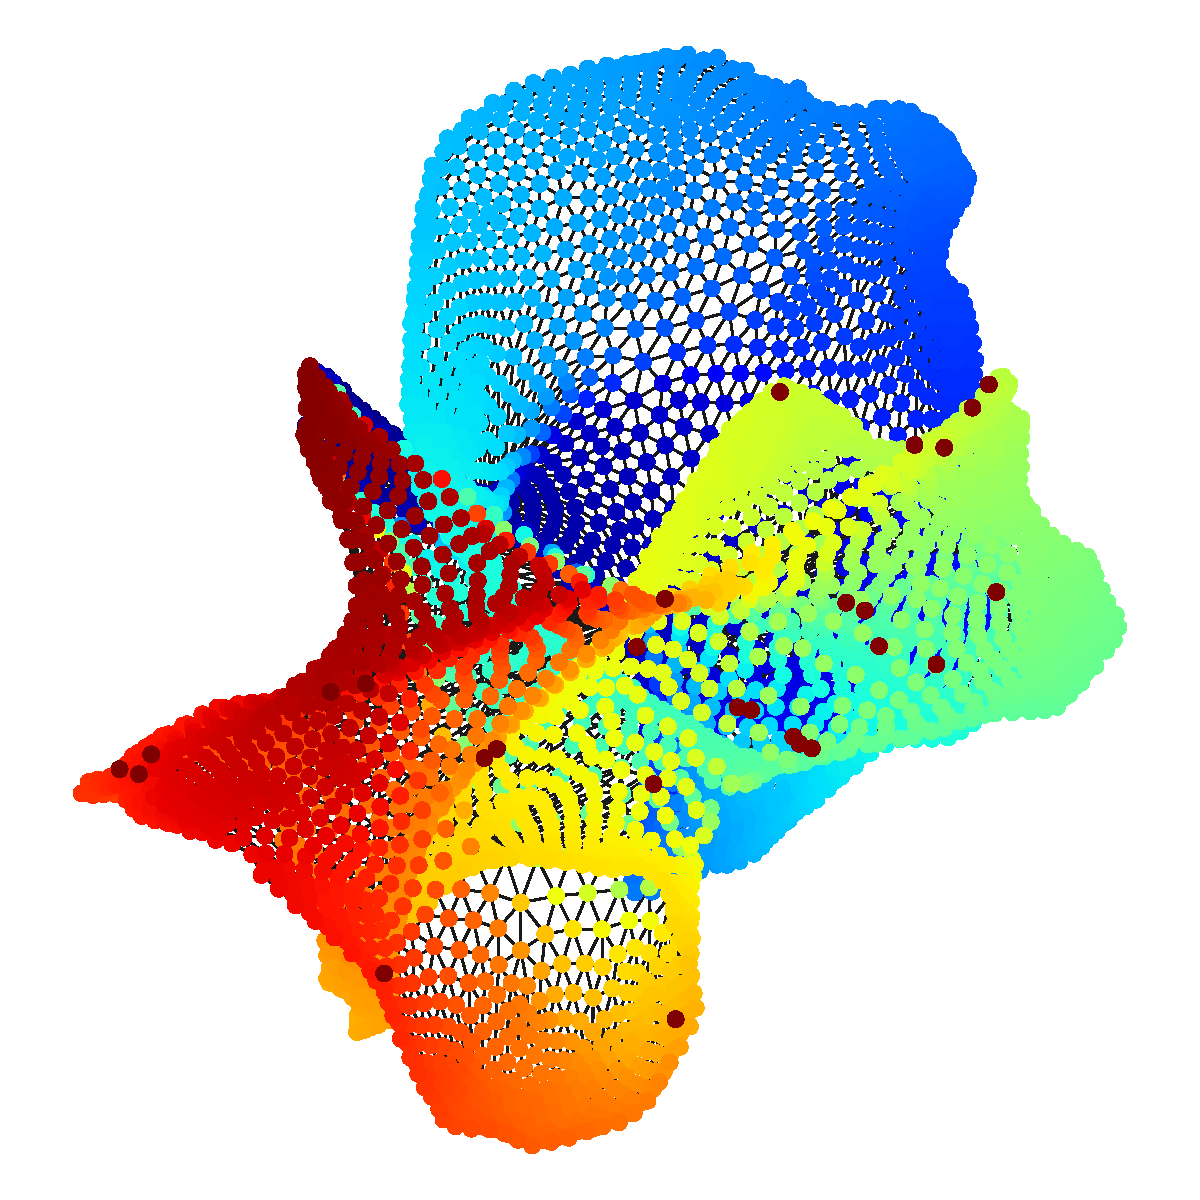
\includegraphics[width=2.5cm]{viz/3elt_L_BFGS.pdf}} &
    \makecell{\scriptsize{RS\_FR}                                       \\[-0.2em]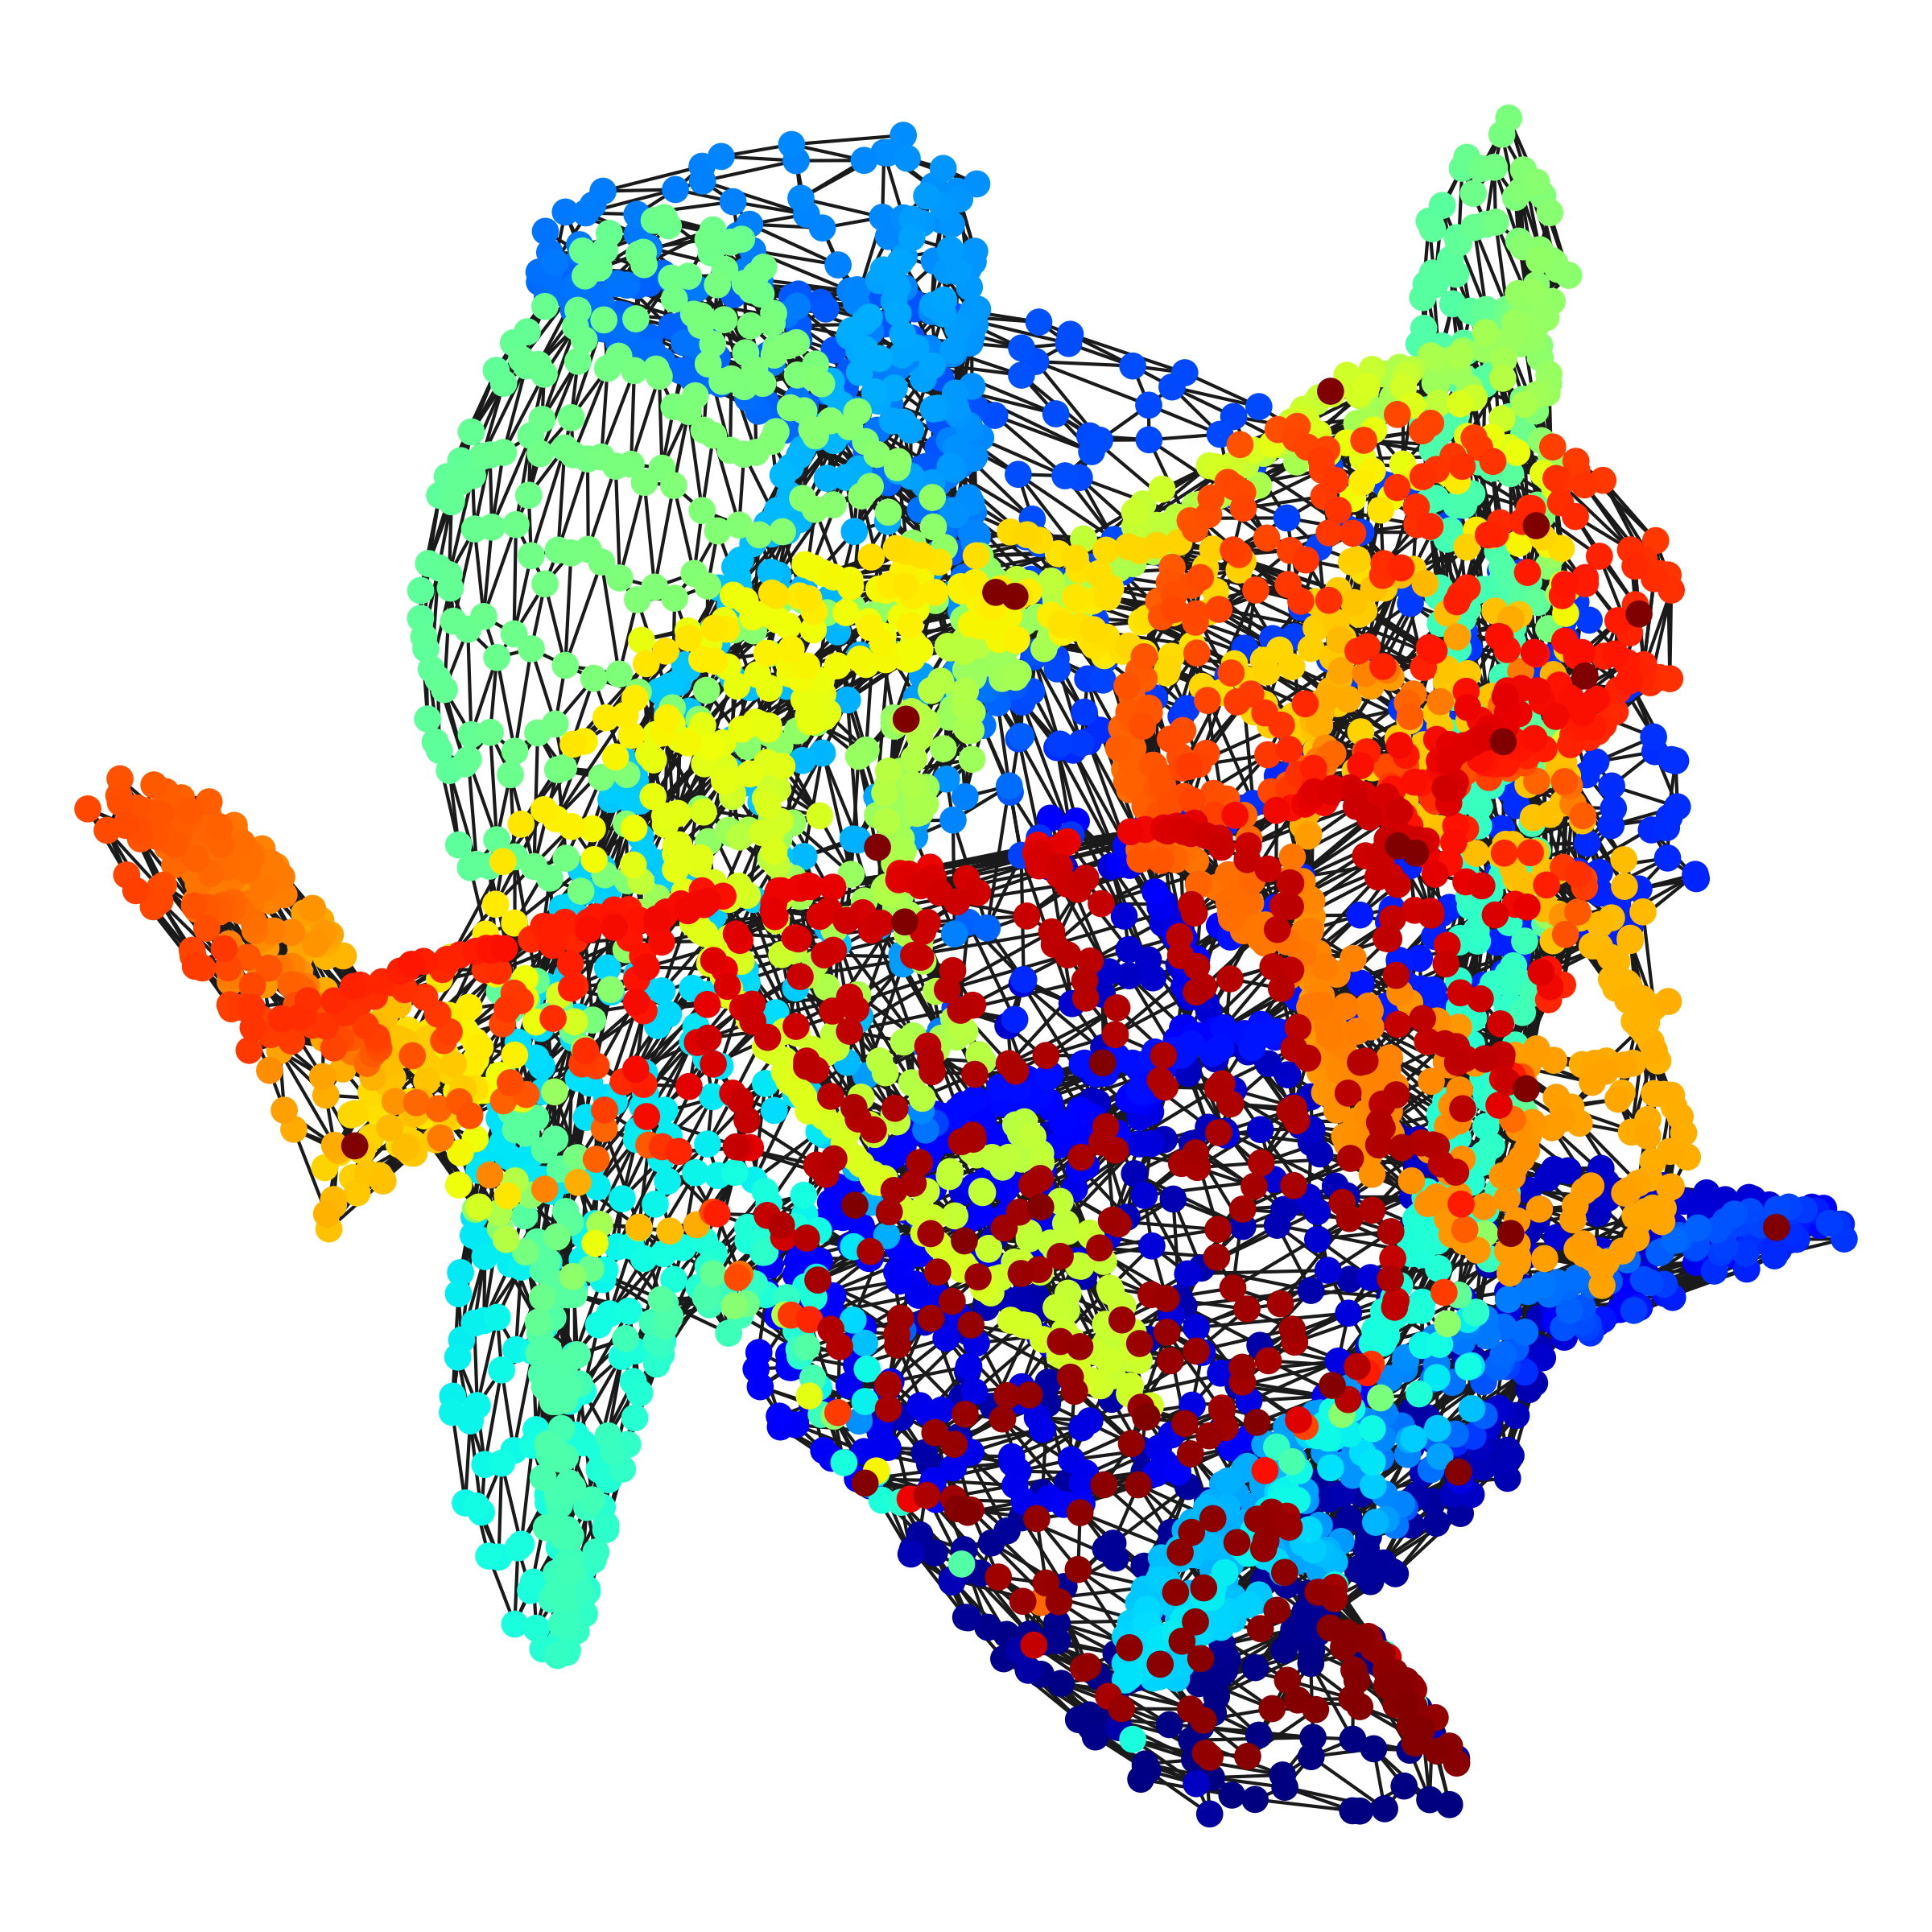
\includegraphics[width=2.5cm]{viz/3elt_RS_FR.pdf}} &
    \makecell{\scriptsize{RS\_L\_BFGS}                                  \\[-0.2em]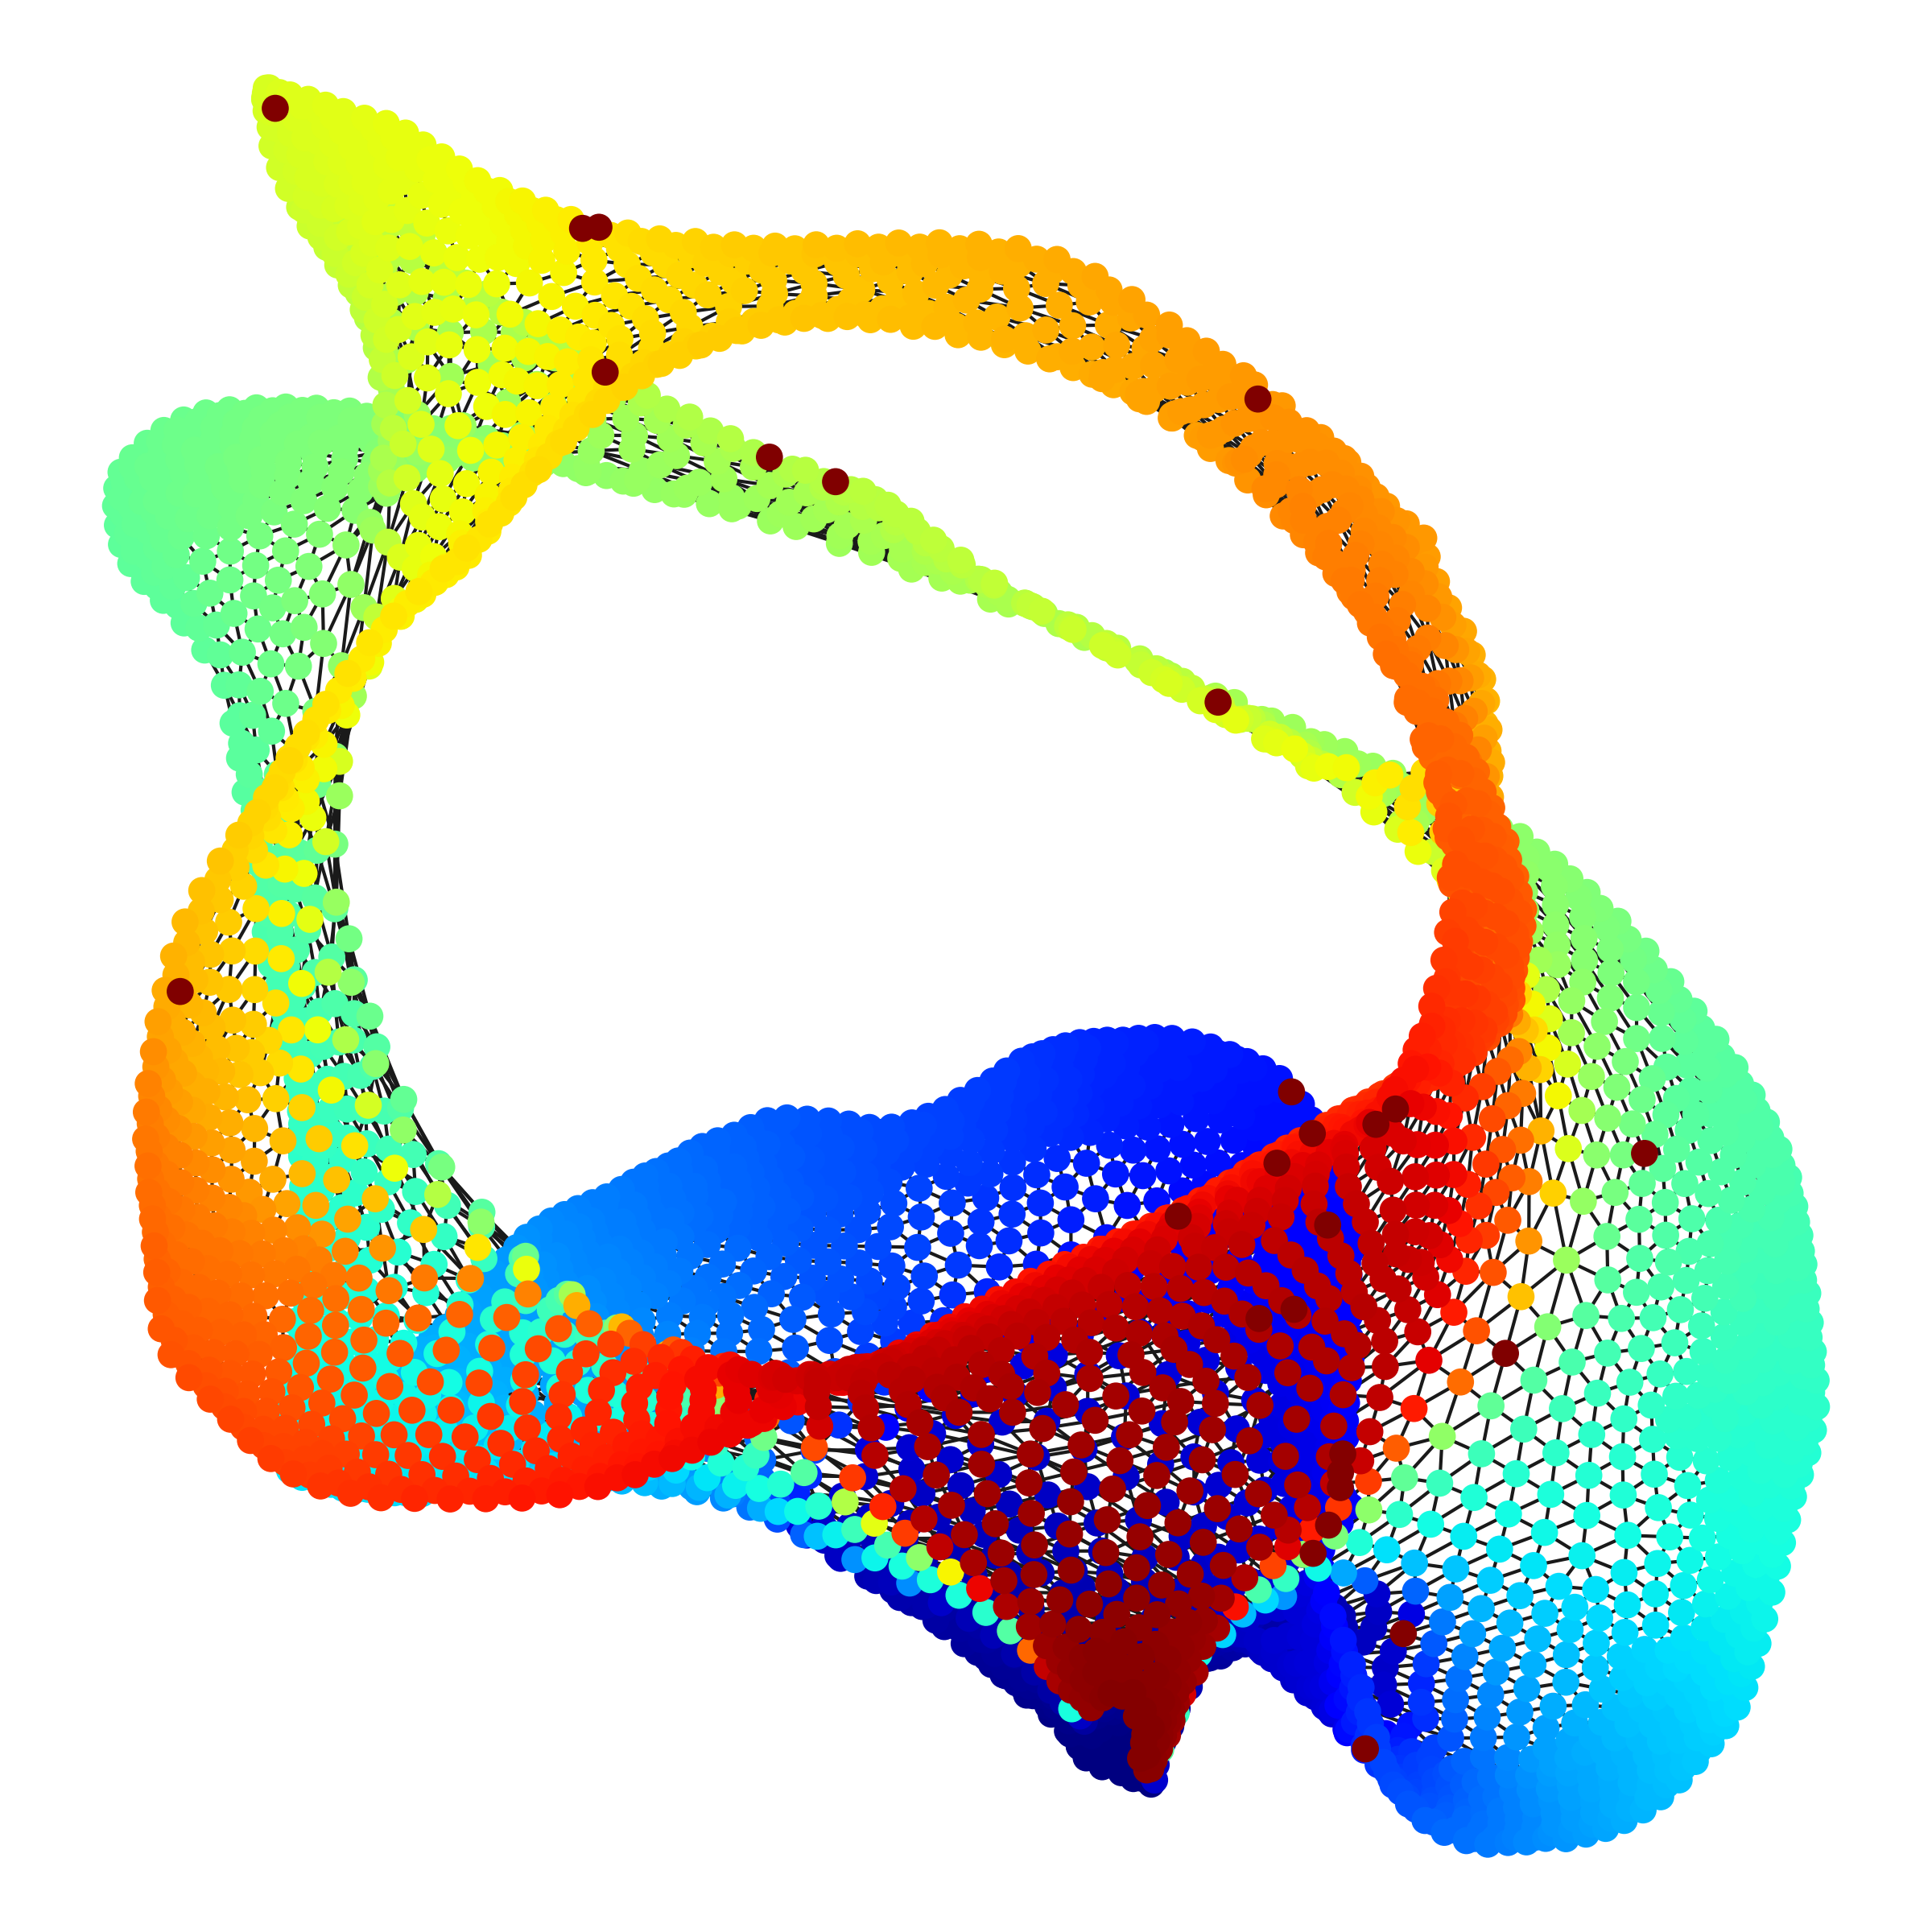
\includegraphics[width=2.5cm]{viz/3elt_RS_L_BFGS.pdf}} \\
  \end{tabular}
\end{table}
\end{document}
